\documentclass[11pt]{article}
\usepackage[a4paper, portrait, margin=1in]{geometry}
\usepackage{graphicx}
\usepackage{hyperref}
\usepackage{caption}
\usepackage[labelformat=simple]{subcaption}    %%Adding option to remove parenthesis
\renewcommand{\thesubfigure}{\normalsize Figure \thefigure. (\alph{subfigure}):}
% \usepackage{subcaption}
% \usepackage{subcaption}
%\usepackage{dirtytalk}
\usepackage{float}
\usepackage{eldar_report}
% Useful packages
\usepackage{amsmath}
% \newcommand\norm[1]{\lVert#1\rVert}
\newcommand\normx[1]{\Vert#1\Vert}
\usepackage{graphicx}
\usepackage{lifetime}
\newcommand{\Dana}[1]{\textcolor{purple}{\bf Dana: #1}}
\newcommand{\Julian}[1]{\textcolor{purple}{\bf Julian: #1}}


\begin{document}

\title{Maximal Robust Layer-Neighborhoods in Multi-Label Neural Networks}

\author{
    \textbf{Julian Mour} \\
    \\
    Advisor: Dana Drachsler Cohen\\
    Technion - Israel Institute of Technology
}

\maketitle

\section{Introduction}

In the last years, many works have demonstrated that deep neural networks (DNNs) are susceptible to a variety of adversarial example attacks, e.g.,~\cite{ref7,ref15,szegedy2014intriguing,ref17,ref29,ref56}.
However, most of the existing work focuses on multi-class, single-label classifiers, where a single instance (e.g.\ an image) is associated with a single label, not mentioning the case of multi-label classifiers where an image can be associated with more than one label.
The association of two or more labels to a single image can be interesting when it comes to the network's vulnerability to perturbations;
How can a perturbed object in an image affect the classification of another?

In this thesis, we want to explore the robustness of different multi-label classifiers in one class - the target class, while adding perturbation around another - the non-target class.
We first build layers around the non-target object in the image.
Each layer can be perturbed by an epsilon (defined specifically for this layer), while maintaining robustness for the target class - not affecting the classification of the target class.
Meaning, we want a sequence of epsilons that for a specific classifier and image, defines a robust layer-neighborhood for the target class.
To get best results, we want the layer-neighborhood to be maximal.


Our key idea is to compute the sequence of epsilons by verifying and optimizing it in each step, rather than computing each epsilon individually.
Given a sequence of epsilons representing an epsilon of perturbation per layer, we check if the layer-neighborhood of a specific image is robust for the target object by running a robustness verifier on it and a specific classifier.
To optimize a robust layer-neighborhood, we compute some gradients in which we can expand our neighborhood and try to keep it robust.
Similarly, we might need to shrink a non-robust layer-neighborhood so that it becomes robust.
The shrinking process can be done in several ways, such as defining a shrinking weight for each layer.
Weights can be fixed (defined by the index of the layer) or not (e.g.\ sensitivity weights).
 
In our preliminary research, we implemented our approach and ran it on part of the DOUBLE-MNIST test dataset.
We ran our program on 3 different CNN multi-label DOUBLE-MNIST classifiers that were trained differently and hence have different defense attributes: No defense, $L_0$ defense and $L_\infty$ defense.
We present the results of the program on each classifier and a single image as a heatmap representing the sequence of epsilons - one epsilon per layer.

In the future, we intend to improve our algorithms to ensure a better execution time and an efficient number of queries.
We as well want to achieve wider robust layer-neighborhoods.
We also hope to achieve a better understanding of the vulnerability of multi-label classifiers to perturbations and the relation between several class objects in a multi-labeled image.

\section{Problem Definition}
In this section, we define the problem we address.

Informally, we are interested in developing an efficient algorithm that given a single image, it returns a robust layer-neighborhood for a target object (target class);
A robust sequence of epsilons each representing the perturbation per layer.
Each layer is defined to be a set of pixels that share the same distance from a specific non-target object (non-target class) in the image.

Formally, Given a classifier $F$, an image $x$ of size $n\times m$ containing two objects: $c_{target}$ and $c_{non-target}$ \textrm{s.t.} $F(x)$ = \{$c_{target}$, $c_{non-target}$\},
we define the set of layers to be:
\begin{gather*}
    $ L_x = \{l_0^x, l_1^x, \ldots, l_r^x\}\\
    \textrm{s.t.} $ l_d^x = \{(i,j) \in $[1,n]\times [1,m]$ \mid dist((i, j), c_{non-target}) = d\}
\end{gather*}

We aim to build a program that returns a sequence of epsilons $(\varepsilon_0^x, \varepsilon_1^x, \ldots, \varepsilon_r^x)$ representing a robust perturbations of the pixels in the corresponding layers for the target class.
Formally:
\begin{gather*}
    $ \varepsilon_x = (\varepsilon_0^x, \varepsilon_1^x, \ldots, \varepsilon_r^x)\\
    \textrm{s.t.} $ \forall x' \in N(x): c_{target} \in F(x')\\
    N(x) = \{x' \mid \forall l_d^x\in L_x: \forall (i,j)\in l_d^x: x'_{i,j} \in [x_{i,j}-\varepsilon_d^x, x_{i,j}+\varepsilon_d^x]\}\\
\end{gather*}

\section{Our Approach}

In this thesis, we will build a program that given a multi-label classifier and an image, can find a layer-neighborhood of the image around a certain object (non-target class) that is robust for another object (target class) in the image.
A straight-forward solution would be to calculate each epsilon individually using a verifier and binary search.
Problem is this approach is very expensive in time hence inefficient.
Our approach aims to reach similar results as the straight-forward one, but in much less time.
In principle, our approach is similar to MaRVeL's~\cite{MARVEL}.
The desired program will have two main components:

\begin{itemize}
    \item The Verifier - The verifier's main job is to check whether a given layer-neighborhood $N(x)$ of an image is robust for the classifier and pass the result to the optimizer.
    Since this is a multi-label classifier, we are interested only in the target class robustness;
    The verifier will say that the neighborhood is robust if and only if all images in the neighborhood are classified to the target class.
    The verifier in our case is a MILP based on the MIPVerify program~\cite{MIPVERIFY} that translates the robustness problem of a multi-label Neural-Network to a MILP maximization problem and uses the Gurobi Optimizer to solve it.
    In addition to checking whether the neighborhood is robust or not, the verifier returns the weakest points of the image.
    These are the points in the checked neighborhood that are least robust and the verifier will pass them to the optimizer as well.
    \item The Optimizer - The optimizer's job is to update a given robust layer-neighborhood by expanding it more, as we intend to maximize the norm of the neighborhood.
    In practice, we try to maximize the norm of the neighborhood and the Robustness Level (RL) of the classifier as well.
    This is done by computing the gradients of both components;
    The norm's gradient is computed in a straightforward way while the RL's gradient is computed using the weakest points found by the verifier.
    At last, we calculate the step gradient, which is a combination of both previous gradients, and expand the neighborhood towards the step gradient.
    If the neighborhood checked by the verifier isn't robust, then we skip the optimization part.
    Instead, we try to minimally shrink the neighborhood so that its robust.
    We do that in two different approaches:
    \begin{itemize}
        \item Fixed weights - We shrink the neighborhood using fixed weights, where we aim to shrink the neighborhood more in layers that are far from the non-target object and less in layers that are close to it.
        \item Sensitivity weights - Similar to the fixed weights approach, but we aim to shrink more in layers that are less sensitive to perturbations.
        We get the sensitivity weights of an image by using the Vanilla Gradient method, introduced by Simonyan et al.~\cite{VANILLAGRADIENT}.
    \end{itemize}
    The new layer-neighborhood will be the input of the verifier in the next iteration.
\end{itemize}
Like that, we do this in iterations many times until convergence of the layer-neighborhood and the RL\@.
We aim to reach a maximal robust layer-neighborhood at the end of the process.


\section{Preliminary Results}
We implemented our approach and ran it on part of the DOUBLE-MNIST test dataset, consisting of images from ten classes;
$C = \{0, 1, \ldots,9\}$ (the 10 different digits), each image classified to two different classes (contains two different digits).
An example of a test dataset sample is shown in Figure~\ref{fig:double-mnist-sample}, where the digit $4$ is the target object and the digit $9$ is the non-target object.
\begin{figure}
    \centering
    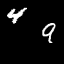
\includegraphics[width=0.4\textwidth]{3.png}
    \caption{DOUBLE-MNIST sample}
    \label{fig:double-mnist-sample}
\end{figure}

We ran our program on 3 different CNN multi-label DOUBLE-MNIST classifiers.
While the three of them solve the same classification problem, they differ in their training process:

\begin{itemize}
    \item Network with no defense - This network is trained regularly on the original DOUBLE-MNIST training dataset, without additional processing done to the training dataset.
    In Figure~\ref{fig:No defense} we present results of our program ran on this classifier and a single image, as a heatmap representing the epsilons per each layer.
    \begin{figure}
         \centering
         \begin{subfigure}[b]{0.4\textwidth}
             \centering
             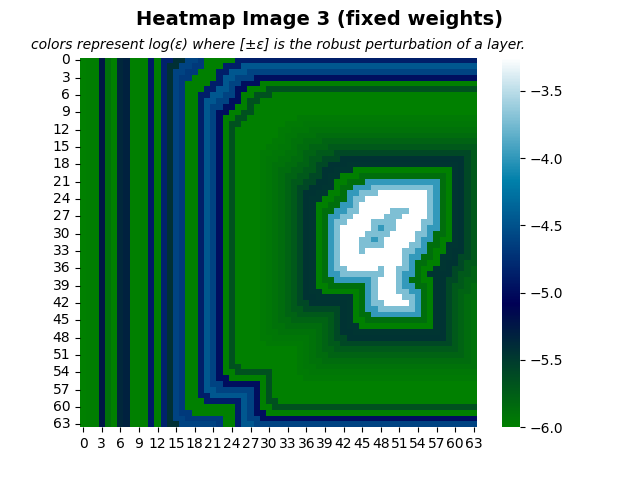
\includegraphics[width=\textwidth]{no_defense_fixed_weights.png}
             \caption{fixed weights}
             \label{sub-fig:No defense FW}
         \end{subfigure}
         \hfill
         \begin{subfigure}[b]{0.4\textwidth}
             \centering
             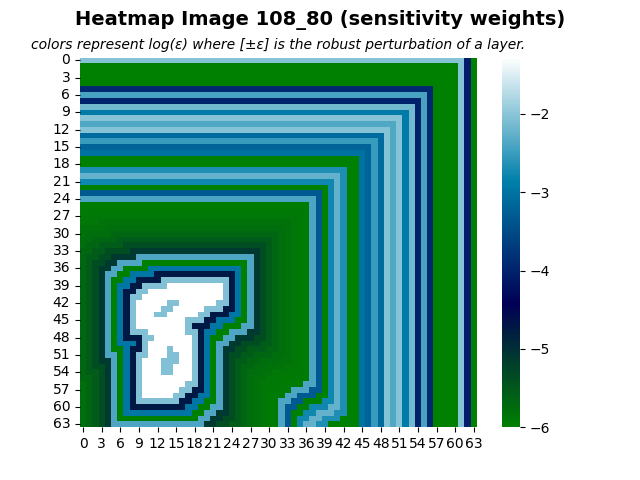
\includegraphics[width=\textwidth]{no_defense_sensitivity_weights.png}
             \caption{sensitivity weights}
             \label{sub-fig:No defense SW}
         \end{subfigure}
         \caption{No Defense}
         \label{fig:No defense}
     \end{figure}
    \item Network with $L_0$ defense - This network is trained with $L_0$ defense.
    To achieve this kind of defense, we add data-augmentation to the process of training;
    Before forwarding a training sample to the network, we add random noise to the image.
    Specifically, we randomly choose a rectangular section in the image and zero all its pixels (color them black).
    In Figure~\ref{fig:L0 defense} we present results of our program ran on this classifier and a single image, as a heatmap representing the epsilons per each layer.
    \begin{figure}
         \centering
         \begin{subfigure}[b]{0.4\textwidth}
             \centering
             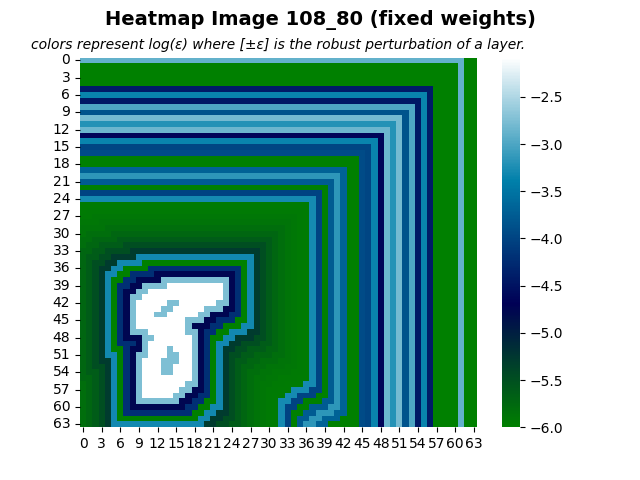
\includegraphics[width=\textwidth]{l0_defense_fixed_weights.png}
             \caption{fixed weights}
             \label{sub-fig:L0 defense FW}
         \end{subfigure}
         \hfill
         \begin{subfigure}[b]{0.4\textwidth}
             \centering
             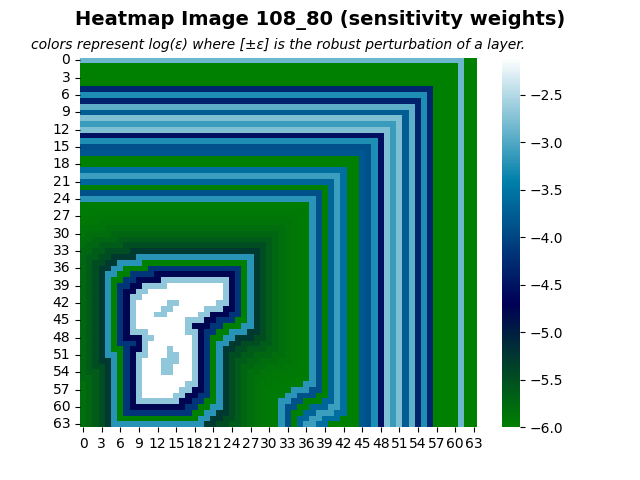
\includegraphics[width=\textwidth]{l0_defense_sensitivity_weights.png}
             \caption{sensitivity weights}
             \label{sub-fig:L0 defense SW}
         \end{subfigure}
         \caption{$L_0$ Defense}
         \label{fig:L0 defense}
    \end{figure}
    \item Network with $L_{\infty}$ defense -
\end{itemize}


\section{Future Research Objectives}
In light of the preliminary work, we aim to further explore our ideas in the following directions:
\begin{itemize}
    \item Improved algorithm: Maximizing the neighborhood norm, execution time and number of queries -
    The main challenge in using our above-mentioned approach is the calculation of the weakest points that are later used by the optimizer to compute the RL gradient.
    Where in the regular single-label case at most $|C|$ queries are executed per iteration to achieve an accurate and unbiased RL gradient, this number jumps to $|C|^2$ in the multi-label case if the same approach as MaRVeL's is used, leading to a much longer execution time.
    Also, we aim to maximize the neighborhood norm;
    We want to achieve wide robust layer-neighborhoods.
    This can be affected by many factors (e.g.\ the shrinking method used in the algorithm) - we will explore each of these factors and look for the best methods to achieve this goal.
    \item Explainability - The goal of our program is to present a relation between two objects in an image for a specific multi-label classifier.
    The results can tell us how much and where we can change in one object so that it doesn't or does affect the other.
    These can vary between different classifiers as well, which will also help us understand which type of multi-label networks are most vulnerable to perturbations in different locations in their inputs.
\end{itemize}

\section{Related Work}
%Our thesis lies at the intersection of adversarial attacks and program synthesis. We next review some
%related work.
%\subsection{Adversarial Attacks}
%Several aspects can be used to classify adversarial attacks~\cite{taxonomy}:
%\begin{itemize}
%    \item Targeted Vs. Untargeted - A targeted attack~\cite{papernot2015limitations} attempts to mislead a classifier by classifying input to a \textit{specific class} that differs from the true class of input.
%    In untargeted attacks~\cite{ref7}, the goal is to cause the classifier to classify the input to \textit{any class} that is different from the true class.
%    \item Individual Vs. Universal - Individual attacks generate different attacks for each different input, by optimizing the attack based on the input~\cite{ref7,papernot2015limitations,moosavidezfooli2016deepfool}.
%    Universal attacks, on the other hand, generate one attack for all possible inputs.
%    Studies from the last few years have indicated that universal adversarial attacks are capable of generalizing well to unseen data.
%    The first method for universal adversarial attack was based on accumulating perturbations iteratively by composing perturbations for each data point~\cite{moosavidezfooli2017universal}.
%    Other studies have used singular vectors~\cite{khrulkov2017art} and networks for adversary generation (NAGs)~\cite{mopuri2018nag}.
%    \item White box Vs. Black box - In white box attacks, the architecture, weights, and parameters of the model are known to the adversary.
%    First, white box adversarial attacks were derived through the generation of artificial perturbations using gradient-based optimization~\cite{szegedy2014intriguing}.
%    There have been numerous works since then that have demonstrated different approaches to generating white-box adversarial attacks, such as FGSM\cite{ref7}, JSMA~\cite{papernot2015limitations}, and Deepfool~\cite{moosavidezfooli2016deepfool}.
%    Attackers using black box methods assume they can only query the model without any further knowledge of it.
%    Several studies have shown that a black-box approach can lead to generating successful attacks~\cite{BlackBox1, BlackBox2, BlackBox3, BlackBox4}.
%\end{itemize}
%
%Additionally, we investigate $L_0$ attacks, which aim to modify a small number of pixels.
%In previous studies, it has been demonstrated that even a single pixel perturbation can lead to successful attacks\cite{OnePixelAttack, alatalo2021chromatic, vargas2019understanding}.
%
%\subsection{Program synthesis}
%Program synthesis is the task of automatically generating a computer program from user requirements.
%It has been studied for decades and shown success in a variety of fields,
%such as data wrangling\cite{inbook}, code repair\cite{d39antoni2016qlose}, code suggestions\cite{10.1145/2594291.2594321}, probabilistic modeling\cite{nori2015efficient} and superoptimization\cite{10.1145/36206.36194}.
%Later, constructive techniques have been developed, such as enumerative
%search\cite{6679385}, programming by examples\cite{inbook}, constraint solving\cite{CSP}, stochastic search\cite{schkufza2012stochastic}, neural program synthesis\cite{parisotto2016neurosymbolic} and genetic programming\cite{Koza92}.
%In our preliminary work, we focused on a variant of genetic search.



\bibliography{bibliography}
\bibliographystyle{plain}

\end{document}
